\section{Introdução}
\par Este relatório, desenvolvido no âmbito da Unidade Curricular de Controlo de Voo aborda a modelação e a síntese de controlo 
para a aeronave Boeing 737, considerando a condição de voo 4, com o objetivo de regular o ângulo de rumo em volta coordenada e 
validar o desempenho numa aterragem no aeroporto London City (LCY). A operação em LCY impõe restrições mais exigentes do que o 
habitual, nomeadamente por requerer aeronaves certificadas para uma ladeira de $5.5\degree$, sendo a simulação iniciada a cerca
de 5 NM da pista, a 2000 ft acima da mesma.

\begin{figure}[hbt!]
    \centering
    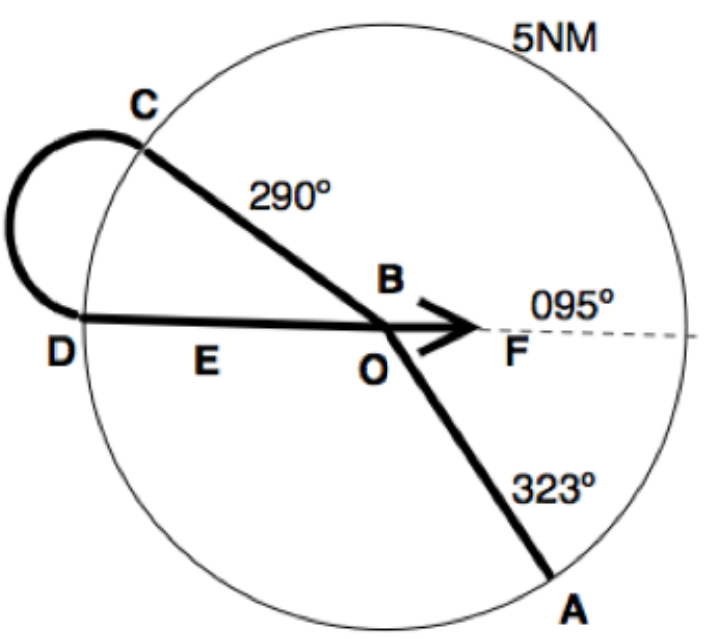
\includegraphics[width=0.45\textwidth]{Body/Images/LCY approach.png}
    \caption{Percurso de volta coordenada considerado, entre os pontos C e D}
    \label{fig:LCY_Approach}
\end{figure}

\par Na condição considerada, a aeronave tem $m = 40 444 \ kg$, pelo que se enquadra na Classe III - avião pesado com 
manobrabilidade moderada - segundo a classificação adotada na UC; por se tratar de uma aterragem, a fase de voo é de 
Categoria C - fase terminal, com manobras lentas e controlo preciso \text{[fazer referência]}. O estudo inclui a obtenção do 
modelo linear relevante e a caracterização das qualidades de voo, a síntese de controladores para estabilização e seguimento do 
rumo em condições próximas de volta coordenada, a integração de sensores e atuadores com limitações realistas, e a validação por 
simulação no cenário de aterragem em LCY.

\section{Determinação e Análise do Modelo Estudado}
\subsection{Formulação do Modelo em Espaço de Estados}

\par Para poder estudar o comportamento da aeronave, é necessário formalizar o seu modelo no espaço de estados. Para tal, recorreram-se às características da aeronave B737 definidas em condição de voo 4 para definir a matriz da dinâmica A e a matriz de entrada B. \textcolor{red}{Temos que elaborar melhor aqui}

\begin{align}
\dot{x} &= A x + B u \\
y &= C x + D u
\end{align}

\par O movimento lateral é descrito, na sua forma geral, pelo vetor de estados $x = [\beta, p, r, \phi, \psi]^T$. No entanto, como o ângulo de guinada $\psi$ é um integrador puro independente dos outros quatro estados, a dinâmica lateral pode ser completamente caracterizada pelo vetor de estados $x = [\beta, p, r, \phi]^T$. Assim sendo, desenvolveu-se a matriz da dinâmica A, tendo em conta a relação $v \approx U_0 \beta$, o que permitiu recorrer às derivadas de $\beta$ disponibilizadas no enunciado: \textcolor{red}{Explicar como calcular os valores com '}

\begin{equation}
A = \begin{bmatrix} Y_\beta & Y_p + W_0 & Y_r-U_0 & g\cos(\theta) \\ L_\beta' & L_p' & L_r' & 0 \\ N_\beta' & N_p' & N_r' & 0 \\ 0 & 1 & \tan(\theta) & 0\end{bmatrix} 
%&= \begin{bmatrix}
%Y_\beta & Y_p + \frac{W_0}{u_0} & Y_r - 1 & \frac{g\cos\theta_0}{u_0} \\
%L_\beta + \frac{I_{xz}}{I_{zz}}N_\beta &
%L_p + \frac{I_{xz}}{I_{zz}}N_p &
%L_r + \frac{I_{xz}}{I_{zz}}N_r &
%0 \\
%N_\beta + \frac{I_{xz}}{I_{zz}}L_\beta &
%N_p + \frac{I_{xz}}{I_{zz}}L_p &
%N_r + \frac{I_{xz}}{I_{zz}}L_r &
%0 \\
%0 & 1 & \tan\theta_0 & 0
%\end{bmatrix}
%\notag
\end{equation}

\begin{equation}
B = \begin{bmatrix} Y_{\delta_A} & Y_{\delta_R} \\ L_{\delta_A}' & L_{\delta_R}'\\ N_{\delta_A}' & N_{\delta_R}'\\ 0 & 0\end{bmatrix}
\end{equation}

Utilizando os valores do enunciado, calculou-se a matriz A: \textcolor{red}{há ali um valor demasiado grande acho eu}

\[
A =
\begin{bmatrix}
-0.0888 & 7.3033\times10^{3} & -1 & 0.1806 \\
-0.6631 & -0.7856 & 0.1759 & 0 \\
0.5677 & -0.0033 & -0.2033 & 0 \\
0 & 1 & 0 & 0
\end{bmatrix}
\]
 
\par Passamos a ter o modelo em espaço de estados:
\begin{equation}
    \dot x = \begin{bmatrix}
-0.0888 & 7.3033\times10^{3} & -1 & 0.1806 \\
-0.6631 & -0.7856 & 0.1759 & 0 \\
0.5677 & -0.0033 & -0.2033 & 0 \\
0 & 1 & 0 & 0
\end{bmatrix} x + \begin{matrix}   \end{matrox}
\end{equation}

\subsection{Análise do Modelo em \textit{Open Loop}}
\begin{table}[h]
\centering
\caption{Lateral Modes and their Characteristics}
\footnotesize
\setlength{\tabcolsep}{7pt}
\begin{tabular}{cccc}
\hline
Polos & $\xi$ & $\omega$ (rad/s) & Modo \\
\hline
$-0.0527$ & 1.0 & 0.0527 & \makecell{Rolamento \\ Puro} \\
$-0.2701 \pm 5.7371i$ & 0.0074 & 69.596 & \makecell{Rolamento \\ Holandês} \\
\hline
\end{tabular}
\end{table}
\textcolor{red}{Explicar o nível dos modos de voo. Verificar se temos mesmo só 2 modos}